\section{PRELIMINARIES}
\label{sec:preliminary}

\subsection{Aging Prediction Model}
\label{subsec:apm}
Before discussing the proposed framework, we briefly introduce the aging (BTI degradation) model for logic gates/networks~\cite{wang2010impact, wang2007efficient, gomez2016early} used in our paper. This model enables us to analyze the long-term behavior of BTI-induced MOSFET degradation, with both aging and recovery mechanisms taken into account. First, the degradation of threshold voltage at a given time $t$ can be predicted as:
\begin{equation}
\label{eq:dtv}
\Delta V_{th\_bti}=\left(\frac{\sqrt{K_v^2 \cdot T_{clk} \cdot \alpha}}{1-\beta_t^{1/_{2n}}}\right)^{2n}
\end{equation}
where $\Delta V_{th\_bti}$ is the BTI-induced $V_{th}$ shift, $K_v$ is a function of threshold voltage ($V_{th}$), temperature, electrical field, and carrier concentration, $\alpha$ is the stress probability, and $n$ is the time exponential constant, 0.2 for the used technology. The detailed explanation of each parameter can be found in~\cite{wang2010impact}. 

Next, as previously indicated in~\cite{wang2010impact, gomez2016early} , the variation in $V_{th}$ can be compensated by the BTI effect. That is, the transistor with a higher (lower) fresh $V_{th}$ ages at a lower (higher) rate and thus, the high $V_{th}$ and the low $V_{th}$ tend to converge toward the nominal case as the stress of BTI continues. The phenomenon is concretely modeled as below~\cite{gomez2016early}:
%Next, the authors of~\cite{gomez2016early} simplify this predictive model to be:
%\begin{equation}
%	\label{eq:dtv2}
%	\Delta V_{th}=b\cdot  \alpha^n \cdot t^n = b \cdot \left(\alpha \cdot t \right)^n
%\end{equation}
%where $b = 3.9 \times 10^{-3} V \cdot s^{-1/5}$.
\begin{equation}
	\centering
	\Delta V_{th\_bti} = (1 - S_{v} \cdot \Delta V_{th\_fresh})  \cdot A \cdot \alpha^n \cdot t^n
	\label{eq:cor}
\end{equation}
where $\Delta V_{th\_fresh}$ is the fresh $V_{th}$ offset (e.g., the offset between high $V_{th}$ and nominal $V_{th}$), $\alpha$ is the stress duty cycle, $A$ is $3.9 \times 10^{-3} V \cdot s^{-1/5}$, $n$ is time exponential constant, 0.2 for used technology, and $S_{v}$ is the sensitivity factor extracted by fitting HSPICE simulation results in 45nm TSMC technology.
Finally, the rising/falling propagation delay of a gate through the degraded P-type/N-type MOSFET can be derived as a first-order approximation:
\begin{equation}
	\label{eq:pd}
	\Delta \tau \propto \Delta V_{th\_bti} + \Delta V_{th\_fresh}
	%\tau^\prime = \tau + a \cdot \left(\alpha \cdot  t\right)^n
\end{equation}
%where $\tau$ is the intrinsic delay of the gate without BTI degradation and $a$ is a constant.
where $\Delta \tau$ is the shift of propagation delay.

We apply Equation (\ref{eq:pd}) to calculate the delay of each gate under BTI, and further estimate the performance of a logic circuit. The coefficient $a$ in Equation (\ref{eq:pd}) for each gate type and each input pin is extracted by fitting HSPICE simulation results in 45nm, Predictive Technology Model (PTM). The simplified long-term model successfully predicts the MOSFET degradation, with less than 5\% loss of accuracy against cycle-by-cycle simulations~\cite{wang2007efficient, wang2010impact, gomez2016early}.

\subsection{Duty-Cycle Converter (DCC)}
\begin{figure}
    \centering
    %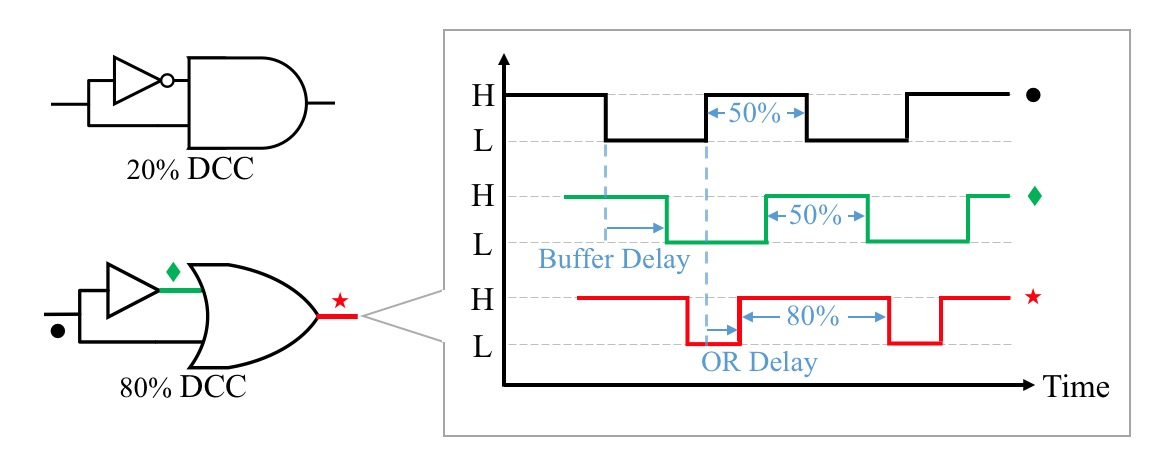
\includegraphics[width=1\columnwidth]{dcc.png} %IEEE Journal
    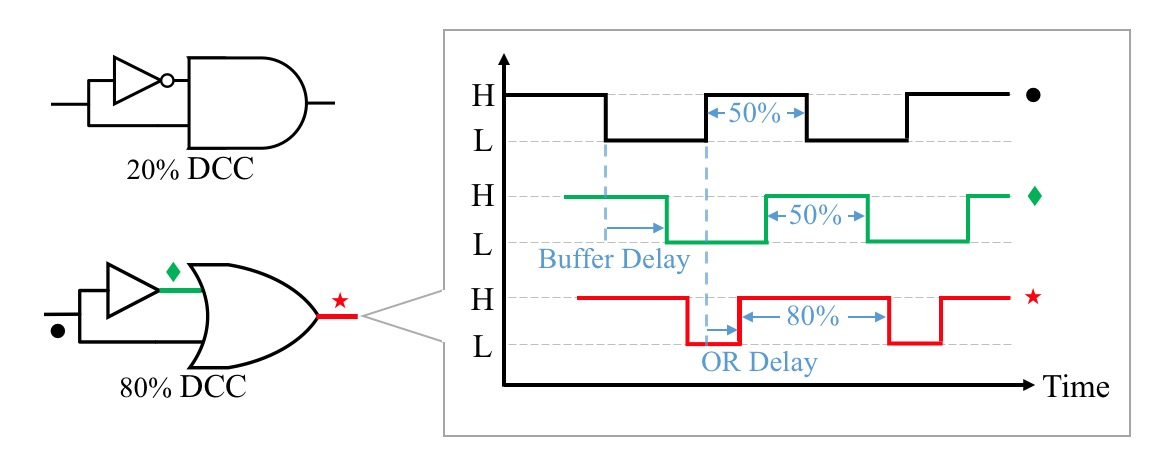
\includegraphics[width=0.7\columnwidth]{dcc.png} %IEEE ACM
    \caption{Construction of DCC and duty-cycle transformation}
    \label{fig:dcc}
\end{figure}

\begin{figure}
    \centering
    %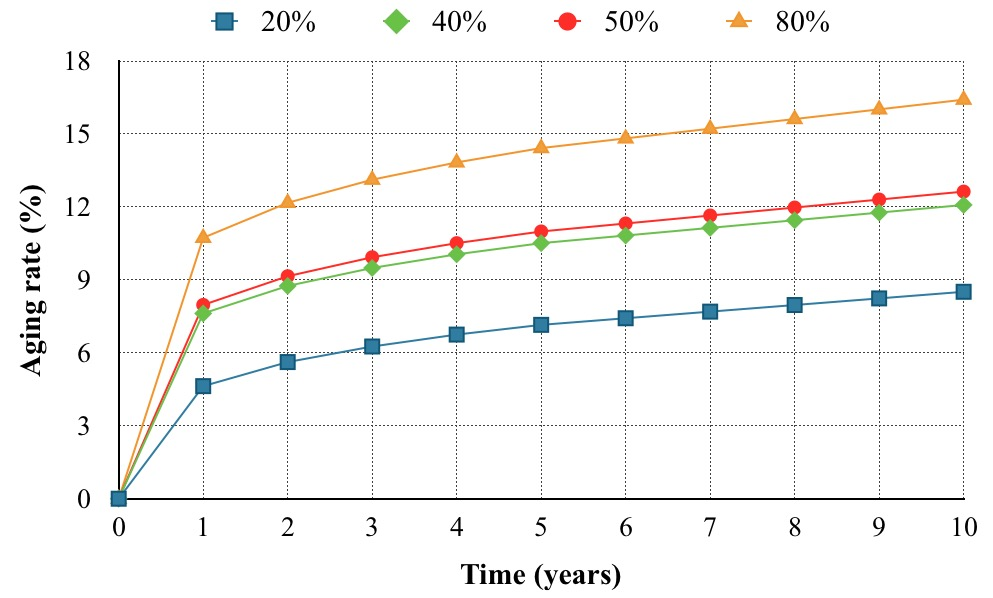
\includegraphics[width=0.9\columnwidth]{agr.png} %IEEE Journal
    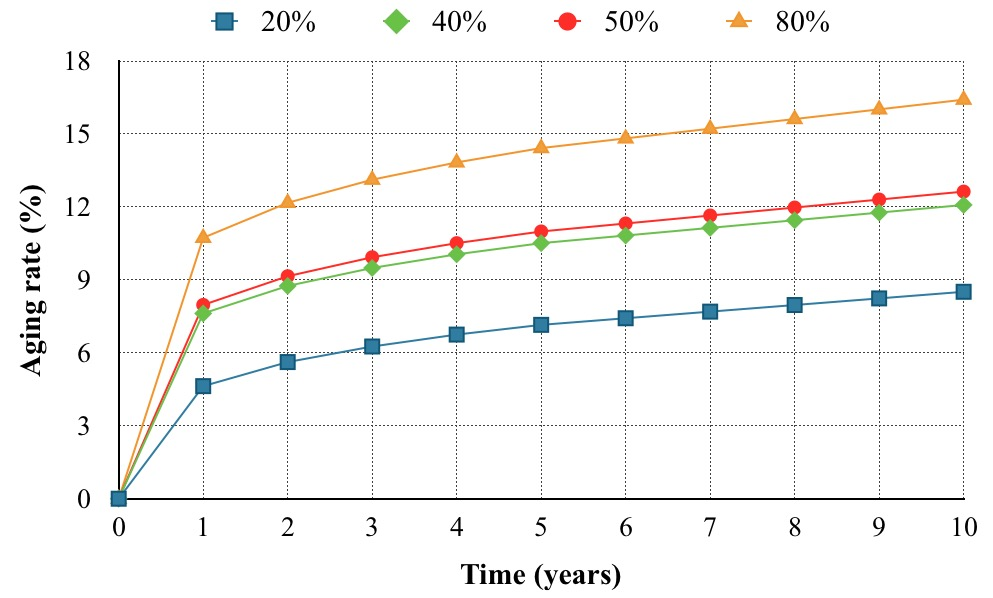
\includegraphics[width=0.65\columnwidth]{agr.png} %IEEE ACM
    \caption{Aging rates of buffers receiving different clock duty cycles}
    \label{fig:agr}
\end{figure}

Duty cycle is the percentage of one period in which a signal is high (i.e., logic 1). The aging of logic gates highly depends on the stress time~\cite{wang2010impact}. For a clock buffer on the clock tree, its stress time is proportional to the clock duty cycle. Therefore, by adjusting the clock duty cycle, we can manipulate the aging of clock buffers and then mitigate the effective degradation of logic paths. Figure~\ref{fig:agr} shows the aging rates of clock buffers receiving different clock duty cycles. 

The unit we use to change the clock duty cycle is duty-cycle converter (DCC), which can converts the duty cycle of a clock signal to a smaller/larger one (e.g., $50\% \rightarrow 20\%$ or $50\% \rightarrow 80\%$), as shown in Figure~\ref{fig:dcc}. Consider the duty-cycle transformation of a clock waveform from 50\% to 80\% as an example, the delayed waveform (green waveform) is separated from the source clock waveform (black waveform). Then, the two waves are combined with the OR gate to obtain a new waveform (red waveform) of 80\% duty cycle. Once a DCC is inserted into the clock tree, the downstream sub-tree of the DCC insertion point will receive a clock signal whose duty cycle is no longer 50\%. This way, aging rate manipulation of downstream clock buffers can be achieved.


\begin{figure}
    \centering
    %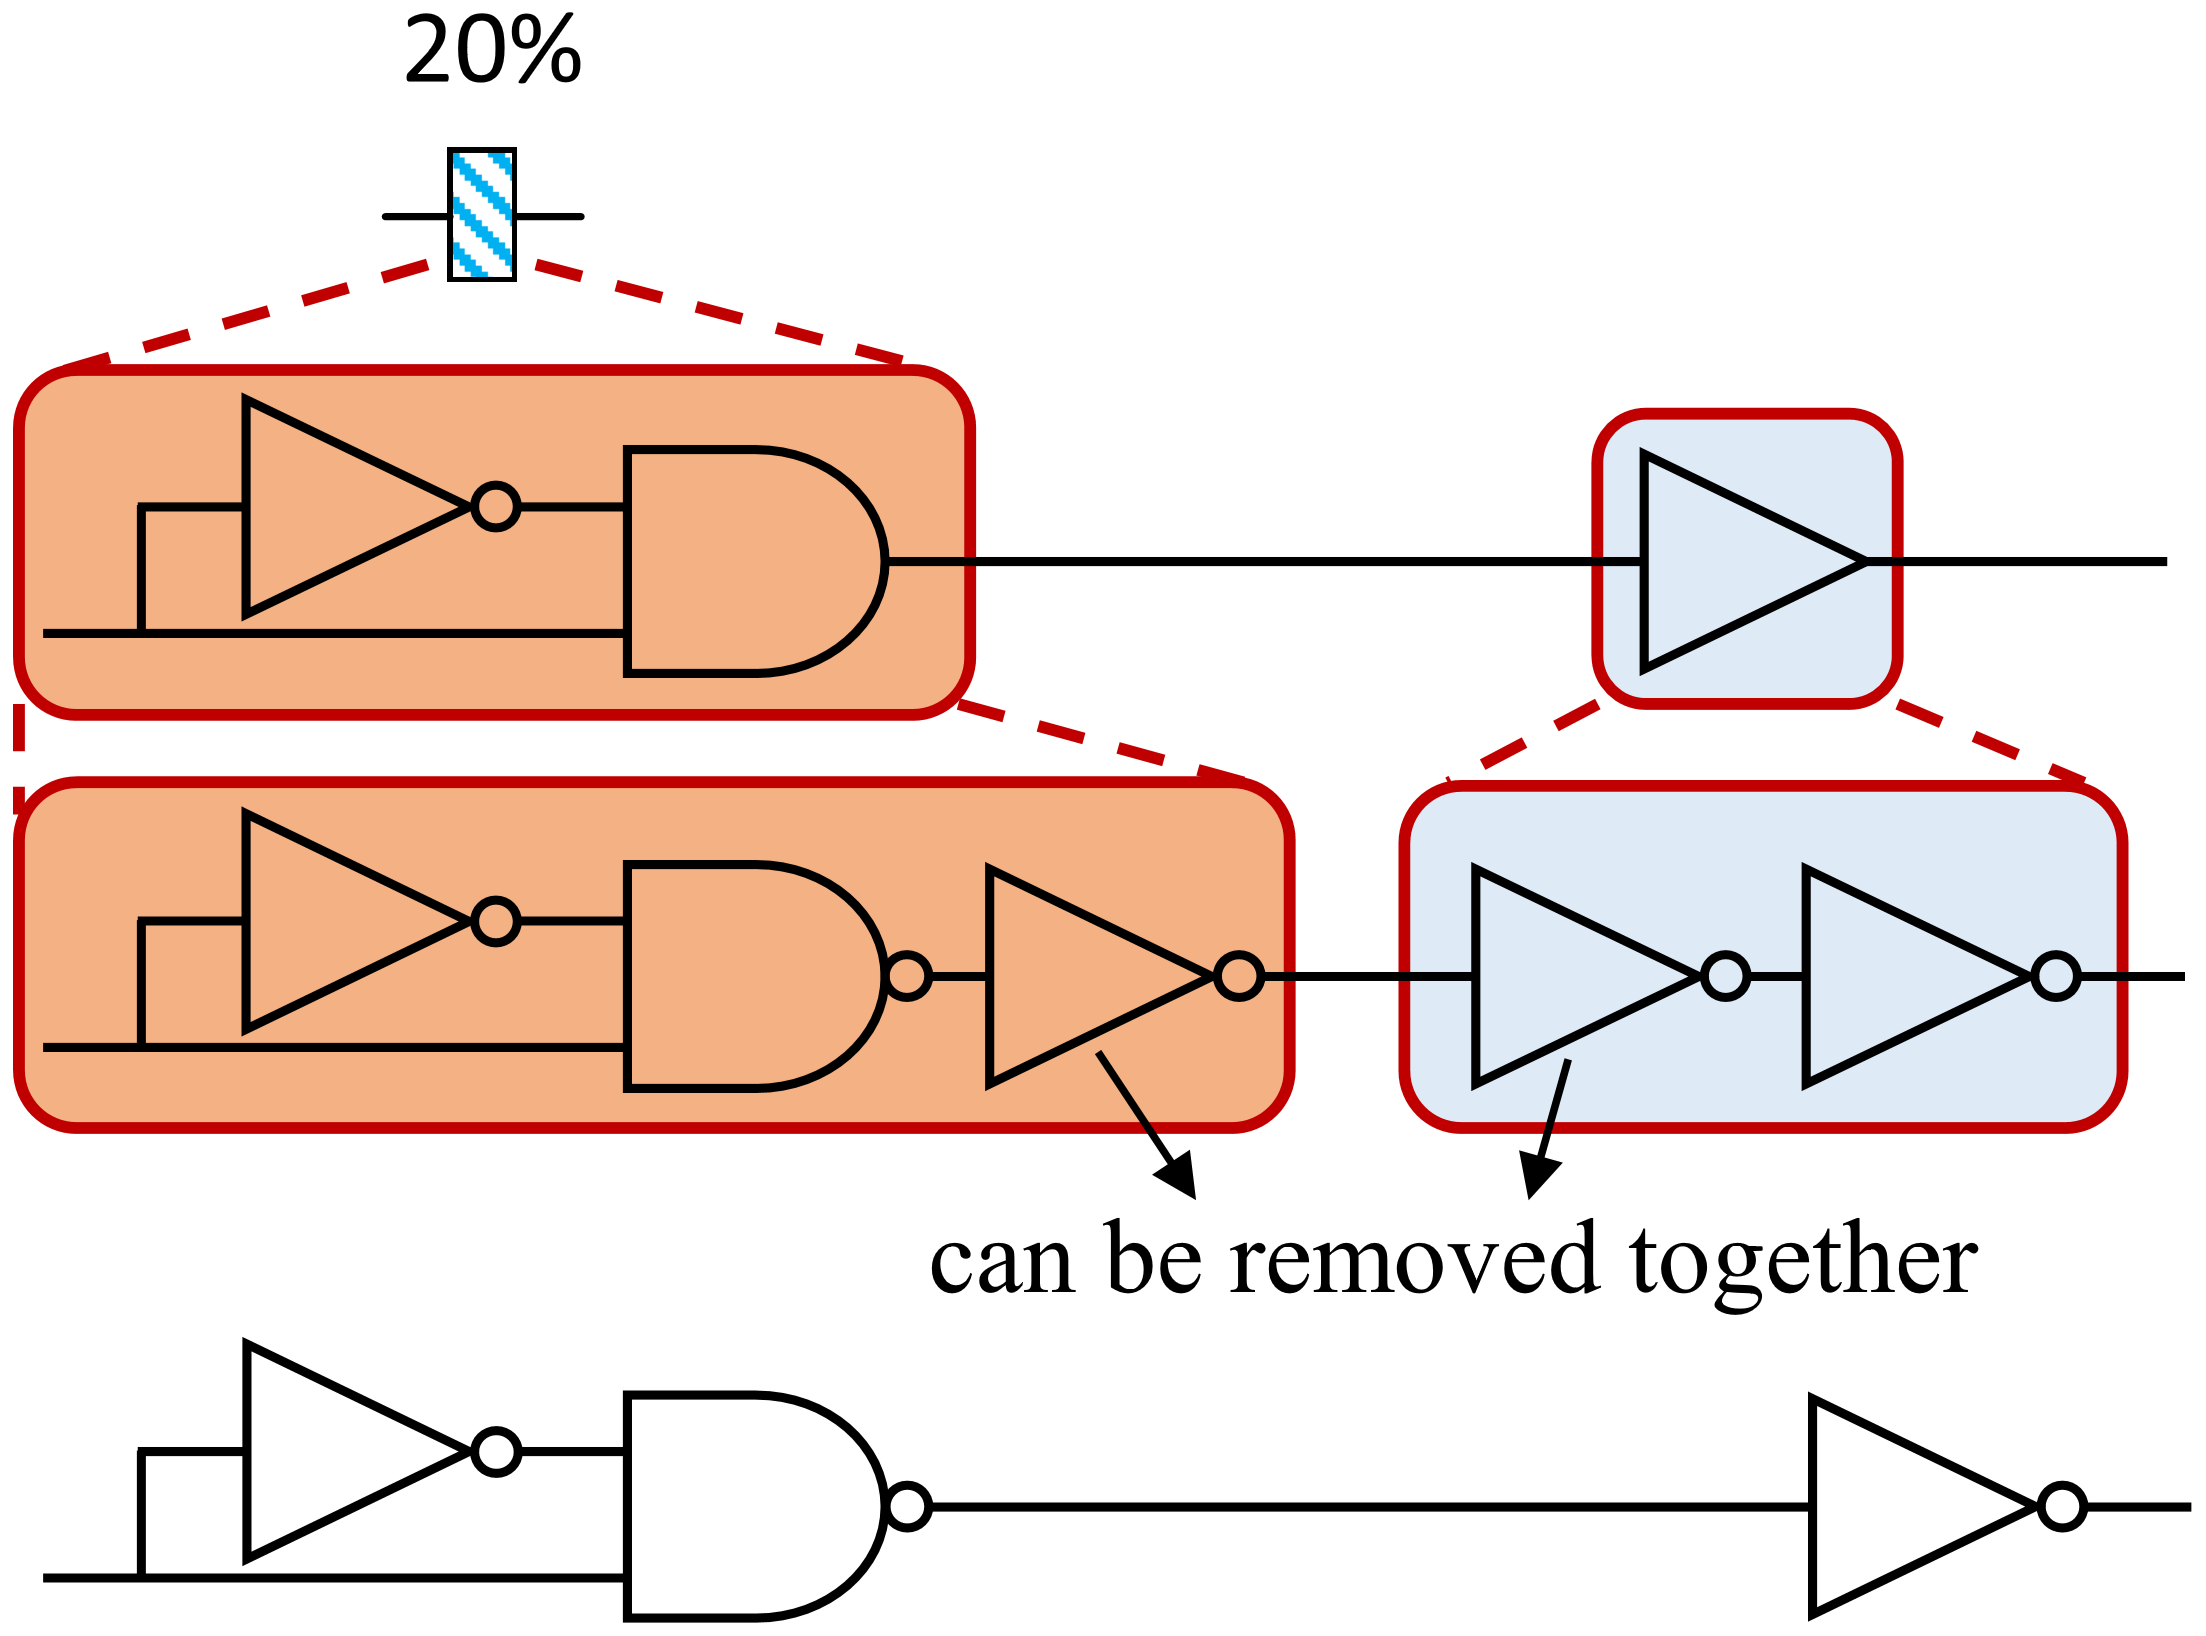
\includegraphics[width=0.5\columnwidth]{DCC_reduction.png} %IEEE Journal
    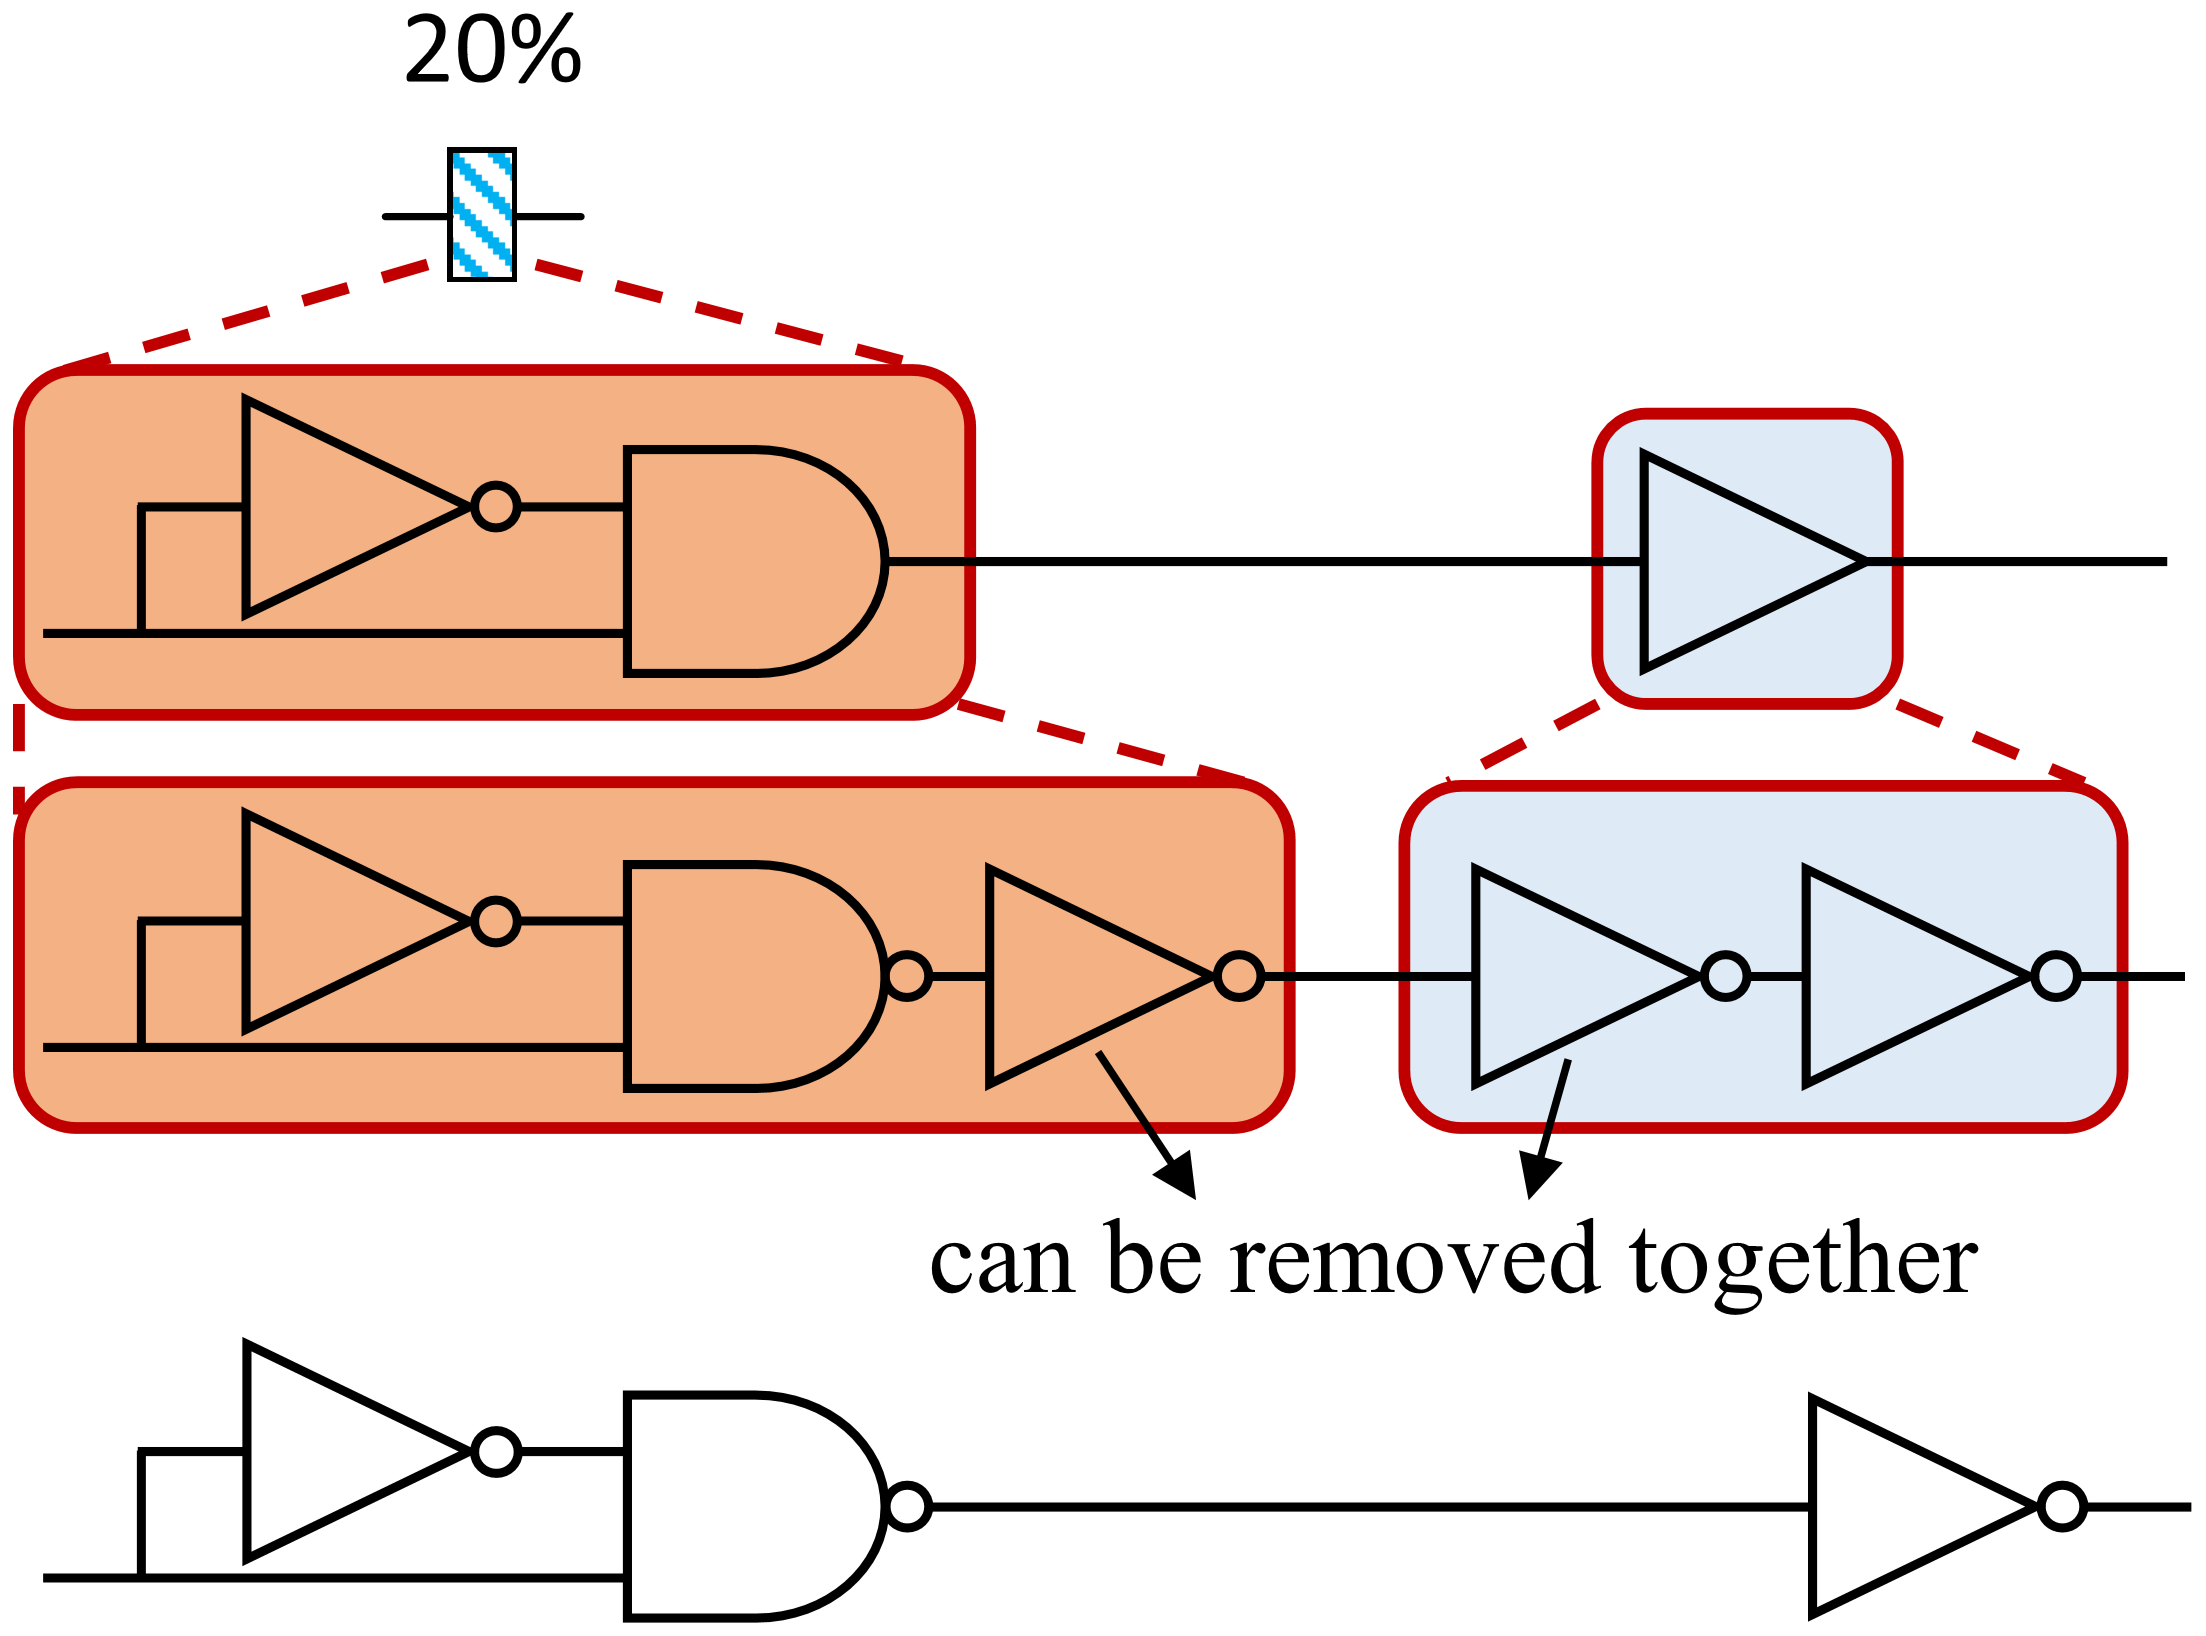
\includegraphics[width=0.4\columnwidth]{DCC_reduction.png} %IEEE ACM
    \caption{Practical considerations for DCC insertion}
    \label{fig:dccreduc}
\end{figure}

\subsection{Practical Considerations}
\label{subsec:tpc}
The diagram on the top of Figure~\ref{fig:dccreduc} shows the primitive design of a DCC, consisting of an inverter and an AND gate. In practice, the AND gate is implemented by a NAND gate feeding an inverter. As mentioned earlier, when inserting a DCC, it is inserted at the input of a buffer, which is a pair of inverters in practice. Therefore, we can actually use the diagram on the bottom of Figure~\ref{fig:dccreduc} to realize the insertion of a DCC. More specifically, we use it as a new cell to \enquote{replace} a buffer when a DCC is needed. By doing so, the cost of a single DCC can be significantly reduced.% and not much more expensive than the cost of inserting a buffer for clock skew scheduling. 
